% !Mode:: "TeX:UTF-8"
% -*-coding: utf-8 -*-

% Русский язык дополнительно настраивать не нужно.
% Убедитесь, что ваш редактор поддерживает UTF-8.
\documentclass{math-mech-sci}

% Название и авторы задаются при помощи специальных
% команд \deftitle и \defauthor. Специальные команды
% требуются для генерации корректной метаинформации в
% PDF-файле.

% Блоки в квадратных скобках опциональны, они предназначены
% для сносок на гранты, которыми поддержана работа.

\usepackage{bm}
\usepackage{subcaption}

\deftitle%
  {О способах выделения сигнала на основе критерия Monte Carlo SSA}

\defauthor%
  {Потешкин Е.П.}%
  {СПбГУ, Санкт-Петербург}%
  {egor.poteshkin@yandex.ru}
\defauthor%
  {Голяндина Н.Э.}%
  {СПбГУ, Санкт-Петербург}%
  {n.golyandina@spbu.ru}

% Электронный адрес у участника пожалуйста укажите один и
% только один, иначе запутается и наш шаблон, и ваш читатель.

\begin{document}

\maketitle

\begin{abstract}
   Рассматриваются методы анализа сингулярного спектра (SSA) и Monte Carlo SSA (MC-SSA) для решения задач обнаружения и выделения сигналов во временных рядах. Предложены три подхода к восстановлению сигнала: адаптивный, полуадаптивный и метод с фиксированной проекцией. Для оценки частоты сигнала используется метод MC-SSA. Проведен численный эксперимент, сравнивающий точность восстановления при различных уровнях шума, типах сигнала и значениях параметра $\delta$, определяющего длину частотного интервала при отборе компонент. Результаты показывают, что полуадаптивный вариант является универсальным выбором, наиболее устойчивым к наличию умеренной амплитудной  модуляции.
\end{abstract}

\section*{Введение}
Рассмотрим следующую модель: $\mathsf{X}=\mathsf{S}+\mathsf{R}$, где $\mathsf{X}$~--- наблюдаемый временной ряд, $\mathsf{S}$~--- сигнал, $\mathsf{R}$~--- шум, т.е. реализация некоторого стационарного процесса. В работе рассматривается две проблемы: проблема обнаружения сигнала $\mathsf{S}$ и проблема выделения сигнала при его наличии.

Для решения первой проблемы используется метод Monte Carlo SSA (MC-SSA)~\cite{AllenSmith96}, проверяющий гипотезу $H_0:\mathsf{S}=0$, а для решения второй~--- метод анализа сингулярного спектра (singular spectrum analysis, SSA)~\cite{Broomhead1986, ssa2001}. Один из шагов SSA подразумевает визуальный анализ для определения компонент сигнала, поэтому возникает потребность в автоматизации этого шага, этой проблеме посвящены, например, работы~\cite{alexandrov,Kalantari2019, circSSA, autoSSA}. Целью работы является определение подходов к автоматическому выделению слабых сигналов, обнаруживаемых критерием MC-SSA, и их сравнение по точности их выделения.

\section*{Метод SSA}
\subsection*{Базовый алгоритм}
Пусть $\mathsf{X}=(x_1,\ldots,x_N)$, $x_i\in \mathbb{R}$,~--- временной ряд длины $N$. Зафиксируем параметр $L$, $1<L<N$, называемый длиной окна и построим так называемую траекторную матрицу $\mathbf{X}=[X_1:\ldots:X_K]$, состоящую из $K=N-L+1$ векторов вложения $X_i=(x_i,\ldots,x_{i+L-1})^{\mathrm{T}}\in \mathbb R^L$.

Следующий шаг~--- разложение в сумму матриц единичного ранга $\mathbf{X}=\sum_{i=1}^d \mathbf{X}_i$. В базовом SSA используется сингулярное разложение матрицы $\mathbf{X}$, где столбцы $\mathbf{X}_i$ состоят из проекций столбцов матрицы $\mathbf{X}$ на порождаемые ею  самой левые сингулярные векторы.

Далее компоненты полученного матричного разложения группируются на основе свойств левых сингулярных векторов, и каждая сгруппированная матрица преобразуется во временной ряд. Таким образом, результатом SSA является разложение временного ряда.

\subsection*{SSA с проекцией}
Метод SSA использует адаптивный базис, но существует возможность зафиксировать некоторые компоненты разложения. Пусть $\mathbf{D}\in\mathbb{R}^{L\times m}$~--- матрица, проекцию на столбцы которой мы хотим зафиксировать в разложении $\mathbf{X}$. Тогда SSA с проекцией отличается от базового алгоритма только шагом разложения:
\begin{enumerate}
    \item В случае, если столбцы матрицы $\mathbf{D}$ не ортонормированны, $\mathbf{D}$ приводится к нужному виду путем ортогонализации Грамма-Шмидта.
    \item Вычисляется матрица $\mathbf{C}=\mathbf{D}\mathbf{D}^\mathrm{T}\mathbf{X}$.
    \item Вычисляется матрица $\mathbf{X}^\star=\mathbf{X}-\mathbf{C}$.
    \item Матрица $\mathbf{X}^\star$ раскладывается в сумму матриц ранга $1$.
\end{enumerate}

\section*{Метод Monte Carlo SSA}
Рассмотрим задачу поиска сигнала во временном ряде. Модель временного ряда имеет вид
\[
    \mathsf{X}=\mathsf{S} + \bm\xi,
\]
где $\mathsf{S}$~--- сигнал, $\bm\xi$~--- стационарный процесс с нулевым средним. Тогда нулевая гипотеза $H_0:\mathsf{S}=0$ и альтернатива $H_1:\mathsf{S}\ne0$.

Зафиксируем длину окна $L$ и обозначим траекторную матрицу ряда $\boldsymbol\xi$ как $\mathbf\Xi$. Рассмотрим вектор $W\in \mathbb R^L$ единичной длины, называемый проекционным вектором. Введем величину
\[
    p=\left\|\mathbf\Xi^{\mathrm{T}} W\right\|^2.
\]
Статистикой критерия является величина
\[
    \widehat p = \left\|{\mathbf{X}}^{\mathrm{T}} W\right\|^2.
\]
Распределение статистики критерия оценивается с помощью моделирования согласно нулевой гипотезе, отсюда и название метода.

Если вектор $W$~--- синусоида с частотой $\omega$, то $\widehat{p}$ отражает вклад частоты $\omega$ в исходный ряд. Так как частота ожидаемого сигнала неизвестна, то необходимо рассматривать несколько векторов $W_k$, $k=1,\ldots,H$. Решение возникающей при этом проблемы множественного тестирования рассматривается в~\cite{Golyandina2023}.
Гипотеза об отсутствии сигнала отвергается, если хотя бы для одного вектора $W=W_k$ значение $\widehat p$ оказывается значимым.

Важной частью метода MC-SSA является способ выбора векторов $W_k$. В данной работе в качестве векторов для проекции берутся косинусы с равноотстоящими частотами $\omega_k=k/(2L)$, $k=1,\ldots,L$. В этом случае можно говорить о значимых частотах, присутствующих в сигнале.

\section*{Подходы к выделению сигнала}
Для ряда $\mathsf{X}$ длины $N$ и $0\leqslant\omega_1\leqslant\omega_2\leqslant0.5$ определим меру, следуя~\cite{alexandrov}
$$
T(\mathsf{X};\omega_1,\omega_2)=\frac{1}{\|\mathsf{X}\|^2}\sum_{k:\omega_1\leqslant k/N\leqslant \omega_2}I_N(k/N),
$$
где $I_N$~--- периодограмма ряда $\mathsf{X}$. Величину $T(\mathsf{X},\omega_1,\omega_2)$ можно рассматривать как долю вклада частот, содержащегося в интервале $[\omega_1,\omega_2]$.

В данной работе будем считать, что сигнал представляет из себя экспоненциально-модулированную гармонику:
$$
\mathsf{S}=\left\{Ae^{\alpha n}\cos(2\pi\omega n)\right\}_{n=1}^N,
$$
где $\omega\in(0, 0.5)$. Пусть $\hat\omega$~--- оценка $\omega$. Обозначим
$$
D_1=\begin{pmatrix}
    \cos(2\pi\hat\omega 1)\\
    \ldots\\
    \cos(2\pi\hat\omega L)
    \end{pmatrix}, \,
D_2=\begin{pmatrix}
    \sin(2\pi\hat\omega 1)\\
    \ldots\\
    \sin(2\pi\hat\omega L)
\end{pmatrix}\in \mathbb{R}^L.
$$
Рассмотрим следующие варианты выделения сигнала $\mathsf{S}$ по частоте $\hat \omega$:
\begin{enumerate}
    \item <<adaptive>>: применить SSA и выбрать первые две компоненты разложения, у которых мера $T$ на интервале $[\hat\omega-\delta, \hat\omega+\delta]$, $\delta>0$, больше некоторого порога $T_0\in[0, 1]$;
    \item  <<semi-adaptive>>: применить SSA с проекцией с $\mathbf{D}=D_1\in \mathbb{R}^{L\times 1}$ и выбрать, помимо компоненты, соответствующей вектору $D_1$, первую компоненту разложения, у которой мера $T$ на интервале $[\hat\omega-\delta, \hat\omega+\delta]$, $\delta>0$, больше некоторого порога $T_0\in[0, 1]$;
    \item <<fixed>>: применить SSA с проекцией с $\mathbf{D}=[D_1:D_2]\in\mathbb{R}^{L\times 2}$ и выбрать компоненты разложения, соответсвующие векторам $D_1$, $D_2$.
\end{enumerate}
Оценивать частоту $\omega$ будем с помощью MC-SSA:
\begin{enumerate}
    \item Найти индекс наиболее значимой частоты, т.е. $k=\operatorname{argmax}_i(\widehat{p}_i-c_i)$, где $c_i$~--- верхняя граница доверительного интервала для $\widehat{p}_i$;
    \item Вычислить значение $\hat\omega$ как взвешенное среднее частот $\omega_{k-1}, \omega_k,\omega_{k+1}$ с весами $w_i=\max(0, \widehat{p}_i-c_i)$;
\end{enumerate}
Такой способ оценки позволяет получить более точную оценку $\omega$ в случае, когда она не попадает в решетку $k/(2L)$.

\subsection*{Численное сравнение подходов}
Проведем численный эксперимент с целью понять, какой из предложенных способов восстановления сигнала наиболее точен. Пусть $N=99$, процесс $\bm\xi$~--- модель AR(1) с параметрами $\phi=0.7$, $\sigma^2\in\{0.2, 0.4, 0.6, 0.8, 1\}$. Для SSA $L=50$, для MC-SSA $L=\widetilde L=40$ (выводы устойчивы к выбору длины окна). В вариантах <<adaptive>> и <<semi-adaptive>> $\delta=0.025$ и $T_0=0.5$. Рассмотрим два типа сигнала $\mathsf{S}$, один из которых является частным случаем другого:
\begin{enumerate}
    % \item $\alpha=0$, $A=1$, $\omega=0.1$.
    \item $\alpha=0$, $A=1$ --- гармоника с постоянной амплитудой.
    % \item $\alpha=0.05$, $A=0.025$, $\omega=0.1$.
    \item $\alpha=0.05$, $A=0.025$ --- экспоненциально-модулированная гармоника.
\end{enumerate}
Возьмем $\omega=0.115$. Заметим, что при таком выборе частоты сигнала $\widetilde L \omega$ не целое, а значит $\omega$ не попадает в решетку $k/(2\widetilde L)$.

На рис.~\ref{fig:mse1} изображена зависимость MSE восстановления сигнала от дисперсии белого шума $\sigma^2$. По графикам видно, что в случае постоянной амлитуды ($\alpha=0$) выигрывает вариант <<fixed>>, однако в случае непостоянной амплитуды фиксированный базис оказывается наихудшим. Полуадаптивный базис, являясь неким компромиссом между адаптивным и фиксированным базисами, оказывается вторым по точности в случае $\alpha=0$ и сравнимым с адаптивным в рассмотренном случае $\alpha\ne0$. При увеличении $|\alpha|$, начиная какого-то момента, фиксированная половина базиса ухудшает восстановление сигнала.

Теперь посмотрим, как будут изменяться ошибки при уменьшении/увеличении $\delta$ для фиксированного $\widetilde L$. На рис.~\ref{fig:mse2} $\delta$ уменьшена, а на рис.~\ref{fig:mse3} увеличена в два раза ($\delta=0.0125$ и $0.05$ соответственно). Из этих графиков видно, что слишком маленькое $\delta$ приводит к ухудшению точности адаптивного и полуадаптивного вариантов в случае $\alpha\ne0$. Связано это с тем, что частота экспоненциально-модулированной гармоники, в отличие от гармоники с постоянной амплитудой, всегда растекается по спектру и чем больше значение показателя экспоненты $\alpha$, тем сильнее это растекание. Увеличение $\delta$ в два раза не привело к значительному изменению точности методов, однако, если и дальше увеличивать $\delta$, ошибки, как и в случае слишком маленького $\delta$, опять возрастут.



\begin{figure}[!h]
    \centering
    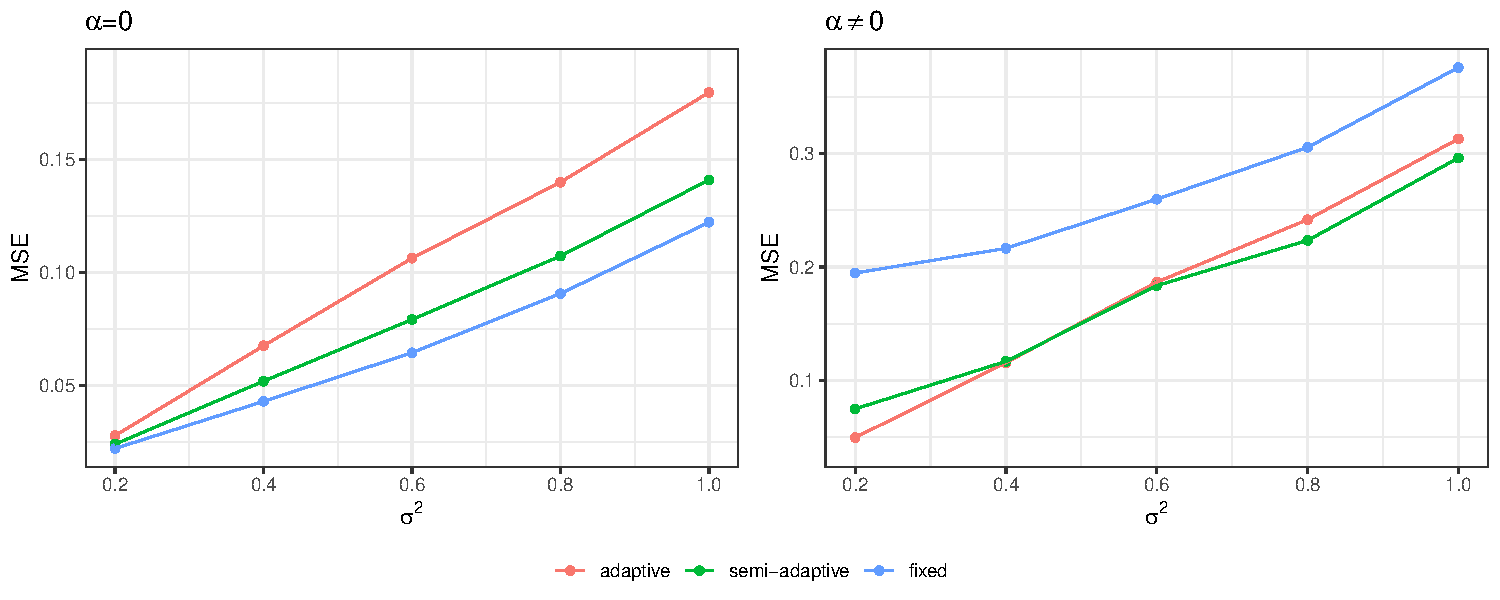
\includegraphics[width=\linewidth]{img/mse.pdf}
    \caption{MSE восстановления сигнала ($\delta=0.025$)}
    \label{fig:mse1}
\end{figure}
\begin{figure}[h!]
    \centering
    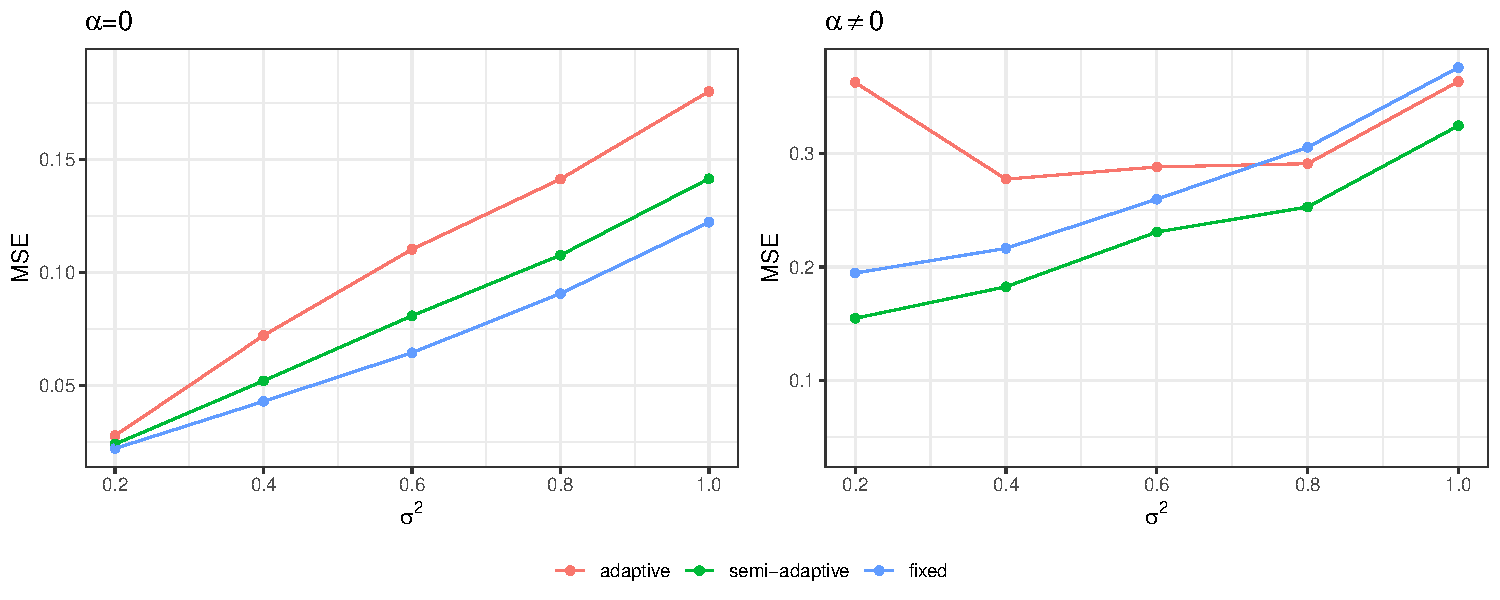
\includegraphics[width=\linewidth]{img/mse_delta_smaller.pdf}
    \caption{MSE восстановления сигнала ($\delta=0.0125$)}
    \label{fig:mse2}
\end{figure}
\begin{figure}[h!]
    \centering
    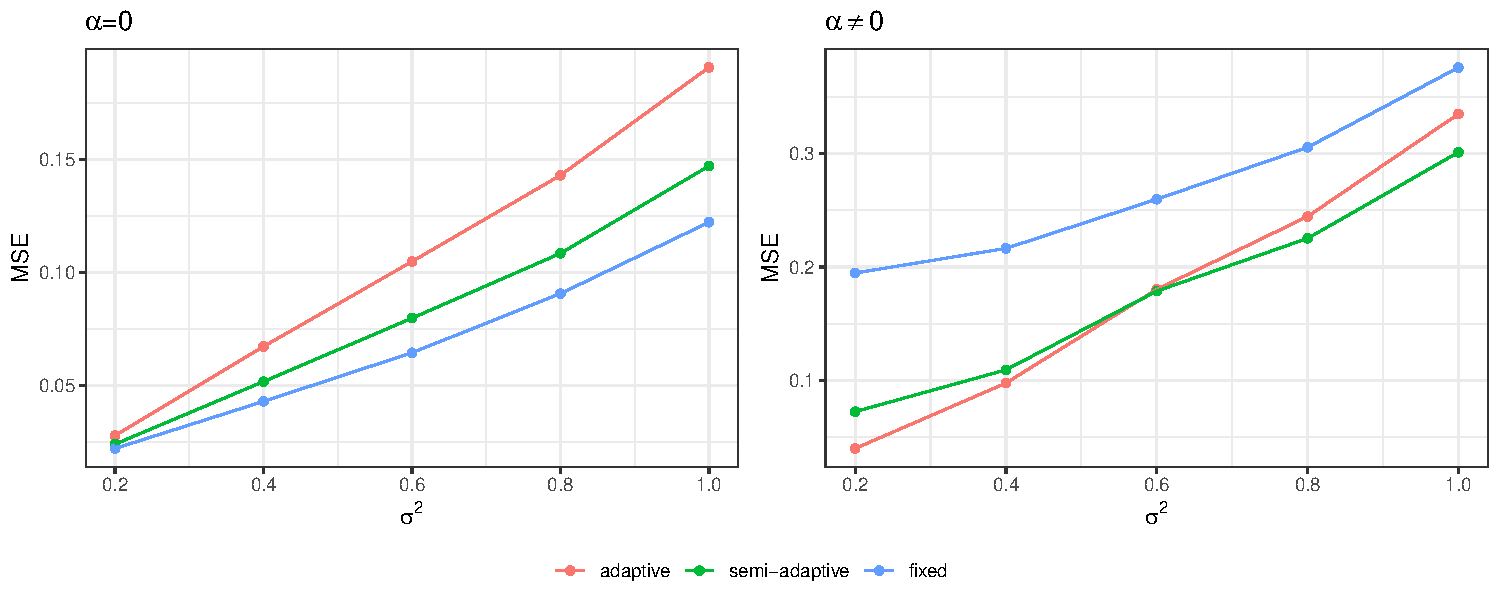
\includegraphics[width=\linewidth]{img/mse_delta_bigger.pdf}
    \caption{MSE восстановления сигнала ($\delta=0.05$)}
    \label{fig:mse3}
\end{figure}



\section*{Заключение}
В статье рассмотрены три подхода к автоматическому выделению сигнала во временных рядах с использованием критерия MC-SSA и метода анализа сингулярного спектра.
% Численные эксперименты показали, что эффективность выделения зависит не только от структуры сигнала и уровня шума, но и от выбора параметра $\delta$, определяющего длину спектрального интервала при отборе компонент. При недостаточно большом $\delta$ адаптивные подходы перестанут обнаруживать нужные компоненты из-за растекания частоты модулированного сигнала, а при слишком большом $\delta$ методы начнут ложно идентицифировать шумовые компоненты.
Исследование показало, что полуадаптивный вариант может быть использован в качестве базового в ситуации, когда неизвестно наличие или отсутствие амплитудной модуляции, при этом модуляция не очень сильная. Для выбора параметра $\delta$ нужно делать предположения о силе модуляции. Заметим, что при выборе длины окна для MC-SSA нужно учитывать сочетание мощности критерия  и точности оценивания частоты.

\begin{thebibliography}{8}
    \bibitem{AllenSmith96} Allen~M., Smith~L. Monte Carlo SSA: detecting irregular oscillations in the presence of coloured noise // Journal of Climate.~--- 1996.~--- Vol.~9.~--- P.~3373--3404.
    \bibitem{Broomhead1986} Broomhead~D., King~G. Extracting qualitative dynamics from experimental data // Physica D: Nonlinear Phenomena.~--- 1986.~--- Vol. 20, no. 2–3.~--- P.~217--236.
    \bibitem{ssa2001} Golyandina~N., Nekrutkin~V., Zhigljavsky~A. Analysis of Time Series Structure: SSA and Related Techniques.~--- Chapman and Hall/CRC, 2001.
    \bibitem{alexandrov} Александров~Ф., Голяндина~Н.
    Автоматизация выделения трендовых и периодических составляющих временного ряда в рамках метода «Гусеница»-SSA // Exponenta Pro (Математика в приложениях).~--- 2004.~--- Vol.~7-80.~--- P.~54--61.
    \bibitem{Kalantari2019} Kalantari~M., Hassani.~H. Automatic grouping in singular spectrum analysis // Forecasting.~--- 2019.~--- Vol. 1, no 1.~--- P.~189--204.
    \bibitem{circSSA} Bogalo~J., Poncela~P., Senra~E. Circulant singular spectrum analysis: A new automated procedure for signal extraction // Signal Processing.~--- 2021.~--- Vol.~179.
    \bibitem{autoSSA} Golyandina~N., Dudnik~P., Shlemov~A. Intelligent Identification of Trend Components in Singular Spectrum Analysis // Algorithms.~--- 2023.~--- Vol. 16.~--- ID 353.
    \bibitem{Golyandina2023} Golyandina~N. Detection of signals by Monte Carlo singular spectrum analysis: multiple testing // Statistics and Its Interface.~--- 2023.~--- Vol.~16. no~1.~--- P.~147--157.
 %   \bibitem{ssaR} Golyandina~N., Korobeynikov~A., Zhigljavsky~A. Singular spectrum analysis with R.~--- Springer, 2018.
\end{thebibliography}

\end{document}
